% SC4021 Chapter 5: Evaluation
\chapter{Evaluation: Precision, Recall, MAP, and NDCG}\label{ch:evaluation}
\begin{center}\small\textit{If you cannot measure ranking quality, you cannot improve it. Precision and recall are the rulers; MAP and NDCG handle many queries and graded truth.}\end{center}

\noindent\fbox{\parbox{\dimexpr\linewidth-2\fboxsep-2\fboxrule}{%
\textbf{From zero: counting correct answers.} We start from a single ranked list, define precision and recall, then average over recall levels and queries (MAP), and finally handle graded relevance with discounted gains (NDCG).}}
\vspace{0.4em}

\section*{Learning Outcomes}
After this chapter you will be able to:
\begin{enumerate}[label=(L\arabic*)]
  \item compute precision, recall, $F_1$, and $P@k$ for a ranked list;
  \item plot the precision--recall curve and define interpolated precision;
  \item compute Average Precision (AP) and Mean Average Precision (MAP);
  \item define DCG and NDCG for graded relevance and compute them;
  \item describe pooling, Cranfield/TREC methodology, and significance.
\end{enumerate}

% ============================================================
\section{Precision and Recall}\label{sec:pr}
\paragraph{Intuition.} For query $q$, let $Rel$ be the set of relevant docs (ground truth, size $R$) and $Ret_k$ the top-$k$ retrieved. Precision is ``how clean is the answer?'' Recall is ``how complete is the answer?'' A system that returns everything has recall $1$ but terrible precision; one that returns one correct doc has precision $1$ but low recall.

\begin{definition}[Precision, Recall, $F_1$, $P@k$]
\begin{align}
\text{Precision }P &= \frac{|Rel\cap Ret|}{|Ret|},\qquad
\text{Recall }R = \frac{|Rel\cap Ret|}{|Rel|},\\
F_1 &= \frac{2PR}{P+R}\ \text{(harmonic mean)},\qquad
P@k &= \text{precision in top }k.
\end{align}
\end{definition}

\begin{example}[Single query]
$R=4$ relevant docs $\{a,b,c,d\}$. System returns $[a, x, b, y, c]$ (top-5, $x,y$ non-relevant). Then $|Rel\cap Ret_5|=3$, $P=3/5=0.6$, $R=3/4=0.75$, $F_1=0.667$, $P@3=2/3=0.667$, $P@5=0.6$. As $k$ increases, precision typically falls and recall rises or stays.
\end{example}

\begin{figure}[h]\centering
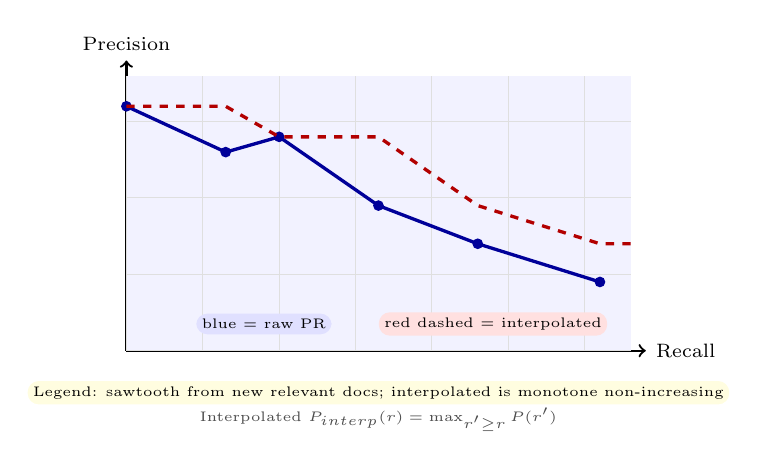
\begin{tikzpicture}[font=\scriptsize, scale=0.97]
  \draw[->, thick] (0,0) -- (6.8,0) node[right] {Recall};
  \draw[->, thick] (0,0) -- (0,3.8) node[above] {Precision};
  \fill[blue!5] (0,0) rectangle (6.6,3.6);
  \draw[gray!25] (0,0) grid (6.6,3.6);
  % raw PR points
  \draw[very thick, blue!60!black] (0,3.2) -- (1.3,2.6) -- (2.0,2.8) -- (3.3,1.9) -- (4.6,1.4) -- (6.2,0.9);
  \foreach \x/\y in {0/3.2, 1.3/2.6, 2.0/2.8, 3.3/1.9, 4.6/1.4, 6.2/0.9} {\fill[blue!60!black] (\x,\y) circle (2pt);}
  % interpolated
  \draw[very thick, red!70!black, dashed] (0,3.2) -- (1.3,3.2) -- (2.0,2.8) -- (3.3,2.8) -- (4.6,1.9) -- (6.2,1.4) -- (6.6,1.4);
  \node[font=\tiny, fill=blue!12, rounded corners, inner sep=2pt] at (1.8,0.35) {blue = raw PR};
  \node[font=\tiny, fill=red!12, rounded corners, inner sep=2pt] at (4.8,0.35) {red dashed = interpolated};
  \node[font=\tiny, fill=yellow!12, rounded corners, inner sep=2pt] at (3.3,-0.55) {Legend: sawtooth from new relevant docs; interpolated is monotone non-increasing};
  \node[font=\tiny, text=gray!60!black] at (3.3,-0.90) {Interpolated $P_{interp}(r)=\max_{r'\ge r} P(r')$};
\end{tikzpicture}
\caption{Precision--recall curve: raw (jagged) and 11-point interpolated (monotone).}
\label{fig:pr-curve}
\end{figure}

\paragraph{Interpolated precision.} IR curves are noisy. Define $P_{interp}(r)=\max_{r'\ge r} P(r')$ -- the best precision achievable at or beyond recall $r$. This makes the curve monotone non-increasing and enables averaging across queries at fixed recall levels (e.g., 11-point: $0,0.1,\dots,1.0$).

% ============================================================
\section{Average Precision and MAP}\label{sec:map}
\paragraph{Intuition.} A single $P@10$ ignores ordering within top-10 and recall beyond. AP rewards putting relevant docs early and accounts for all relevant docs.

\begin{definition}[AP and MAP]
For query $q$ with $R_q$ relevant docs, let $rel(k)=1$ if doc at rank $k$ is relevant else $0$. Then
\begin{equation}
AP(q)=\frac{1}{R_q}\sum_{k=1}^{n} P@k \times rel(k).
\end{equation}
Only ranks where $rel(k)=1$ contribute, weighted by precision there. For a set of queries $Q$,
\begin{equation}
MAP=\frac{1}{|Q|}\sum_{q\in Q} AP(q).
\end{equation}
If a relevant doc is never retrieved, its contribution is $0$.
\end{definition}

\begin{example}[AP by hand]
Relevant $\{a,b,c\}$ ($R=3$). Ranking: $[a, x, b, y, c, z]$ ($x,y,z$ non-rel). Then $P@1=1$, $P@3=2/3$, $P@5=3/5$. So $AP=(1 + 2/3 + 3/5)/3=(1+0.667+0.6)/3=0.756$. If ranking were $[x, a, y, b, z, c]$: $P@2=0.5$, $P@4=0.5$, $P@6=0.5$, $AP=(0.5+0.5+0.5)/3=0.5$ -- lower because relevant docs appear later.
\end{example}

\begin{lstlisting}[language=Python, caption={Precision, recall, and AP for a single query.}, label={lst:ap}]
def precision_recall(retrieved, relevant, k=None):
    if k is not None: retrieved = retrieved[:k]
    tp = len(set(retrieved) & set(relevant))
    prec = tp / len(retrieved) if retrieved else 0
    rec = tp / len(relevant) if relevant else 0
    return prec, rec

def average_precision(retrieved, relevant):
    relevant = set(relevant)
    R = len(relevant)
    ap_sum, hits = 0.0, 0
    for k, doc in enumerate(retrieved, 1):
        if doc in relevant:
            hits += 1
            ap_sum += hits / k  # P@k at relevant rank
    return ap_sum / R if R else 0

rel = {"a","b","c"}
ret = ["a","x","b","y","c","z"]
print("P@3", precision_recall(ret, rel, k=3))
print("AP", round(average_precision(ret, rel),3))  # 0.756
ret2 = ["x","a","y","b","z","c"]
print("AP bad order", round(average_precision(ret2, rel),3))  # 0.5
\end{lstlisting}

% ============================================================
\section{Graded Relevance: DCG and NDCG}\label{sec:ndcg}
Binary relevant/non-relevant is coarse. Real judgments are graded (0=non, 1=marginal, 2=fair, 3=highly relevant). NDCG rewards putting highly relevant docs at the very top, with a discount for lower ranks.

\begin{definition}[DCG / NDCG]
For graded relevance $rel_i$ at rank $i$,
\begin{equation}
DCG@k = \sum_{i=1}^{k} \frac{2^{rel_i}-1}{\log_2(i+1)}\quad\text{or simpler}\quad \sum_{i=1}^{k}\frac{rel_i}{\log_2(i+1)}.
\end{equation}
The exponential numerator emphasises highly relevant. Ideal $IDCG@k$ is DCG@k for docs sorted by $rel$ descending. Then
\begin{equation}
NDCG@k = \frac{DCG@k}{IDCG@k}\in[0,1].
\end{equation}
\end{definition}

\begin{example}[NDCG]
Grades for top-5: $[3,0,2,1,0]$. $DCG@5 = (7/\log2)+(0)+(3/\log4)+(1/\log5)+0 =7/1+3/2+1/2.32=9.93$ (using $2^{rel}-1$). Ideal order $[3,2,1,0,0]$: $IDCG=7/1+3/1.58+1/2=10.58$. $NDCG=0.94$ -- near ideal despite zeros because top doc is highly relevant.
\end{example}

\begin{figure}[h]\centering
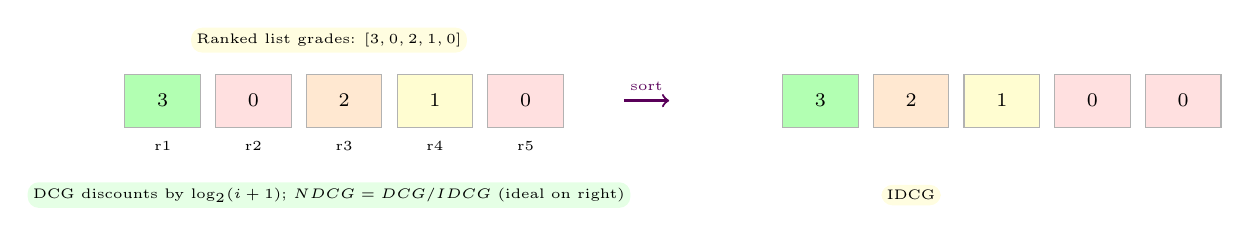
\begin{tikzpicture}[font=\scriptsize, scale=0.96]
  \foreach \i/\g/\col in {1/3/green!30, 2/0/red!12, 3/2/orange!18, 4/1/yellow!18, 5/0/red!12} {
    \fill[\col, draw=gray!60] (1.2*\i,0) rectangle ++(1.0,0.7);
    \node at (1.2*\i+0.5,0.35) {\g};
    \node[font=\tiny] at (1.2*\i+0.5,-0.25) {r\i};
  }
  \node[font=\tiny, fill=yellow!12, rounded corners, inner sep=2pt] at (3.9,1.15) {Ranked list grades: $[3,0,2,1,0]$};
  \draw[->, thick, violet!70!black] (7.8,0.35) -- (8.4,0.35) node[midway, above, font=\tiny] {sort};
  \foreach \i/\g/\col in {1/3/green!30, 2/2/orange!18, 3/1/yellow!18, 4/0/red!12, 5/0/red!12} {
    \fill[\col, draw=gray!60] (8.7+1.2*\i,0) rectangle ++(1.0,0.7);
    \node at (8.7+1.2*\i+0.5,0.35) {\g};
  }
  \node[font=\tiny, fill=green!10, rounded corners, inner sep=2pt] at (3.9,-0.90) {DCG discounts by $\log_2(i+1)$; $NDCG=DCG/IDCG$ (ideal on right)};
  \node[font=\tiny, fill=yellow!12, rounded corners, inner sep=2pt] at (11.6,-0.90) {IDCG};
\end{tikzpicture}
\caption{DCG: grades in ranked order vs.\ ideal order; discount penalises inversions.}
\label{fig:dcg}
\end{figure}

\begin{lstlisting}[language=Python, caption={DCG and NDCG with the exponential gain.}, label={lst:ndcg}]
import math
def dcg(grades, k=None):
    if k is not None: grades = grades[:k]
    return sum((2**g - 1)/math.log2(i+2) for i,g in enumerate(grades))

grades = [3,0,2,1,0]
print("DCG@5", round(dcg(grades),3))
ideal = sorted(grades, reverse=True)
print("IDCG@5", round(dcg(ideal),3))
print("NDCG@5", round(dcg(grades)/dcg(ideal),3))  # 0.939
# Compare a worse ranking: highly relevant at rank 5
bad = [0,0,1,2,3]
print("NDCG bad", round(dcg(bad)/dcg(ideal),3))  # much lower
\end{lstlisting}

% ============================================================
\section{Cranfield, Pooling, and Significance}\label{sec:cranfield}
Real collections are too large to judge exhaustively. TREC/Cranfield methodology: assemble systems, pool their top-$k$ (e.g., top-100 per query across systems), judge only pooled docs, treat unjudged as non-relevant. This biases evaluation against systems that did not contribute to the pool but works well when pools are deep and metrics like MAP/NDCG@10 focus on early ranks. Always report significance (paired t-test or randomization) over queries -- a 0.02 MAP gain may be noise with 10 queries but real with 50.

\begin{figure}[h]\centering
\begin{tikzpicture}[font=\scriptsize, >=Stealth, scale=0.97]
  \node[draw, fill=blue!12, thick, rounded corners, minimum width=2.0cm, minimum height=0.9cm,align=center] (sys) at (0,0) {Systems\\{\tiny submit top-100}};
  \node[draw, fill=yellow!16, thick, rounded corners, minimum width=2.2cm, minimum height=0.9cm,align=center] (pool) at (3.4,0) {Pool\\{\tiny union}};
  \node[draw, fill=green!14, thick, rounded corners, minimum width=2.2cm, minimum height=0.9cm,align=center] (judge) at (6.8,0) {Judges\\{\tiny label rel}};
  \node[draw, fill=violet!14, thick, rounded corners, minimum width=2.2cm, minimum height=0.9cm,align=center] (metric) at (10.2,0) {Metrics\\{\tiny MAP/NDCG}};
  \foreach \a/\b in {sys/pool,pool/judge,judge/metric} \draw[->, thick, blue!60!black] (\a) -- (\b);
  \node[font=\tiny, fill=red!10, rounded corners, inner sep=2pt] at (3.4,-1.05) {unpooled $\to$ assumed non-relevant};
  \node[font=\tiny, fill=yellow!12, rounded corners, inner sep=2pt] at (5.1,-1.50) {Legend: blue=submission, yellow=pool, green=judgment, violet=evaluation};
\end{tikzpicture}
\caption{Pooling for large collections: judge only what systems retrieve near the top.}
\label{fig:pooling}
\end{figure}

% ============================================================

% ============================================================
\section{Micro vs.\ Macro and User-Oriented Metrics}\label{sec:micro-macro}
\paragraph{Intuition.} MAP is macro-averaged (average per query, then mean). Micro-averaged precision pools all query-doc pairs together, giving larger queries more weight. TREC uses macro -- each information need counts equally, not each relevant doc. For imbalanced query sets (some queries have 5 relevant, others 500), the choice flips system rankings.

\paragraph{Other metrics.} $MRR$ (Mean Reciprocal Rank) cares only about the first relevant: $RR=1/rank_{first}$. Good for known-item search (``find the homepage''). Success@k is binary: did we get at least one relevant in top-$k$? For user studies, time-to-first-relevant and effort (clicks) matter more than abstract precision.

\begin{remark}[Statistical testing]
With $|Q|=50$ queries, a MAP difference of 0.03 may be noise. Use paired t-test, Wilcoxon, or randomization (Fisher) over per-query AP differences. Report $p<0.05$ and effect size, not just raw MAP. Bootstrap confidence intervals over queries are increasingly standard.
\end{remark}

\section{Chapter Notes}
MAP was the TREC workhorse for binary judgments; NDCG (J\"arvelin \& Kek\"al\"ainen, 2002) is now standard for graded and top-heavy evaluation. Report $P@10$ and $NDCG@10$ for user-facing quality, MAP for recall-oriented tasks. Always average over queries, not over docs -- queries are the experimental units. See Ch.~8 for how these metrics become training objectives.

% ============================================================
\section{Exercises}
\begin{enumerate}[label=E5.\arabic*, leftmargin=*, itemsep=0.6em]
  \item \textbf{$P,R,F_1$.} $Rel=\{1,2,3,4,5\}$, $Ret=[1,6,2,7,3]$. Compute $P$, $R$, $F_1$, $P@3$, $R@3$. If you add doc $4$ at rank 6, how do $P$ and $R$ change?
  \item \textbf{PR curve.} Relevant $\{a,b,c\}$. Ranking $[a,x,b,y,c]$. Compute $P@k$ and $R@k$ at each $k$, plot, and compute 11-point interpolated precision at $r=0,0.5,1.0$.
  \item \textbf{AP/MAP.} Two queries: $q_1$ rel $\{a,b\}$, ret $[a,x,b]$; $q_2$ rel $\{c,d,e\}$, ret $[x,c,y,d,z,e]$. Compute $AP(q_1)$, $AP(q_2)$, $MAP$. Which query is harder?
  \item \textbf{NDCG.} Grades top-4: $[2,0,3,1]$. Compute $DCG@4$ (exponential gain) and $NDCG@4$. What ranking would give $NDCG=1$? Swap ranks 1 and 3, recompute $NDCG$ and quantify the drop.
  \item \textbf{Pooling bias.} A new system retrieves doc $d_{new}$ at rank 2 that no pooled system found. Under ``unjudged = non-relevant,'' what is its $NDCG$ effect? Propose two ways to mitigate pool bias when evaluating novel systems.
\end{enumerate}

